\documentclass[UKenglish, aspectratio = 169]{beamer}

\usepackage{listings}
\usetheme{OsloMet}
\usepackage{style}
\usepackage{dcolumn}

\hidelogo
\author
{Xiaomin Li \texorpdfstring{\\}{} Nina Solovyeva}
\title{Saliency and valuation in decisions}
\subtitle{- an online behavioral experiment}


\begin{document}


% Use
%
%     \begin{frame}[allowframebreaks]
%
% if the TOC does not fit one frame.
\begin{frame}{Table of contents}
    \tableofcontents
\end{frame}




%% Disable the logo in the lower right corner:

\section{Motivation}
\begin{frame}{Research Question}
\begin{itemize}
	\item 
\end{itemize}
\end{frame}

%% Enable the logo in the lower right corner:
\showlogo


\section{Designs and Experiments}
\subsection{Experiment Design}
\begin{frame}{Experiment Design}
	\center
    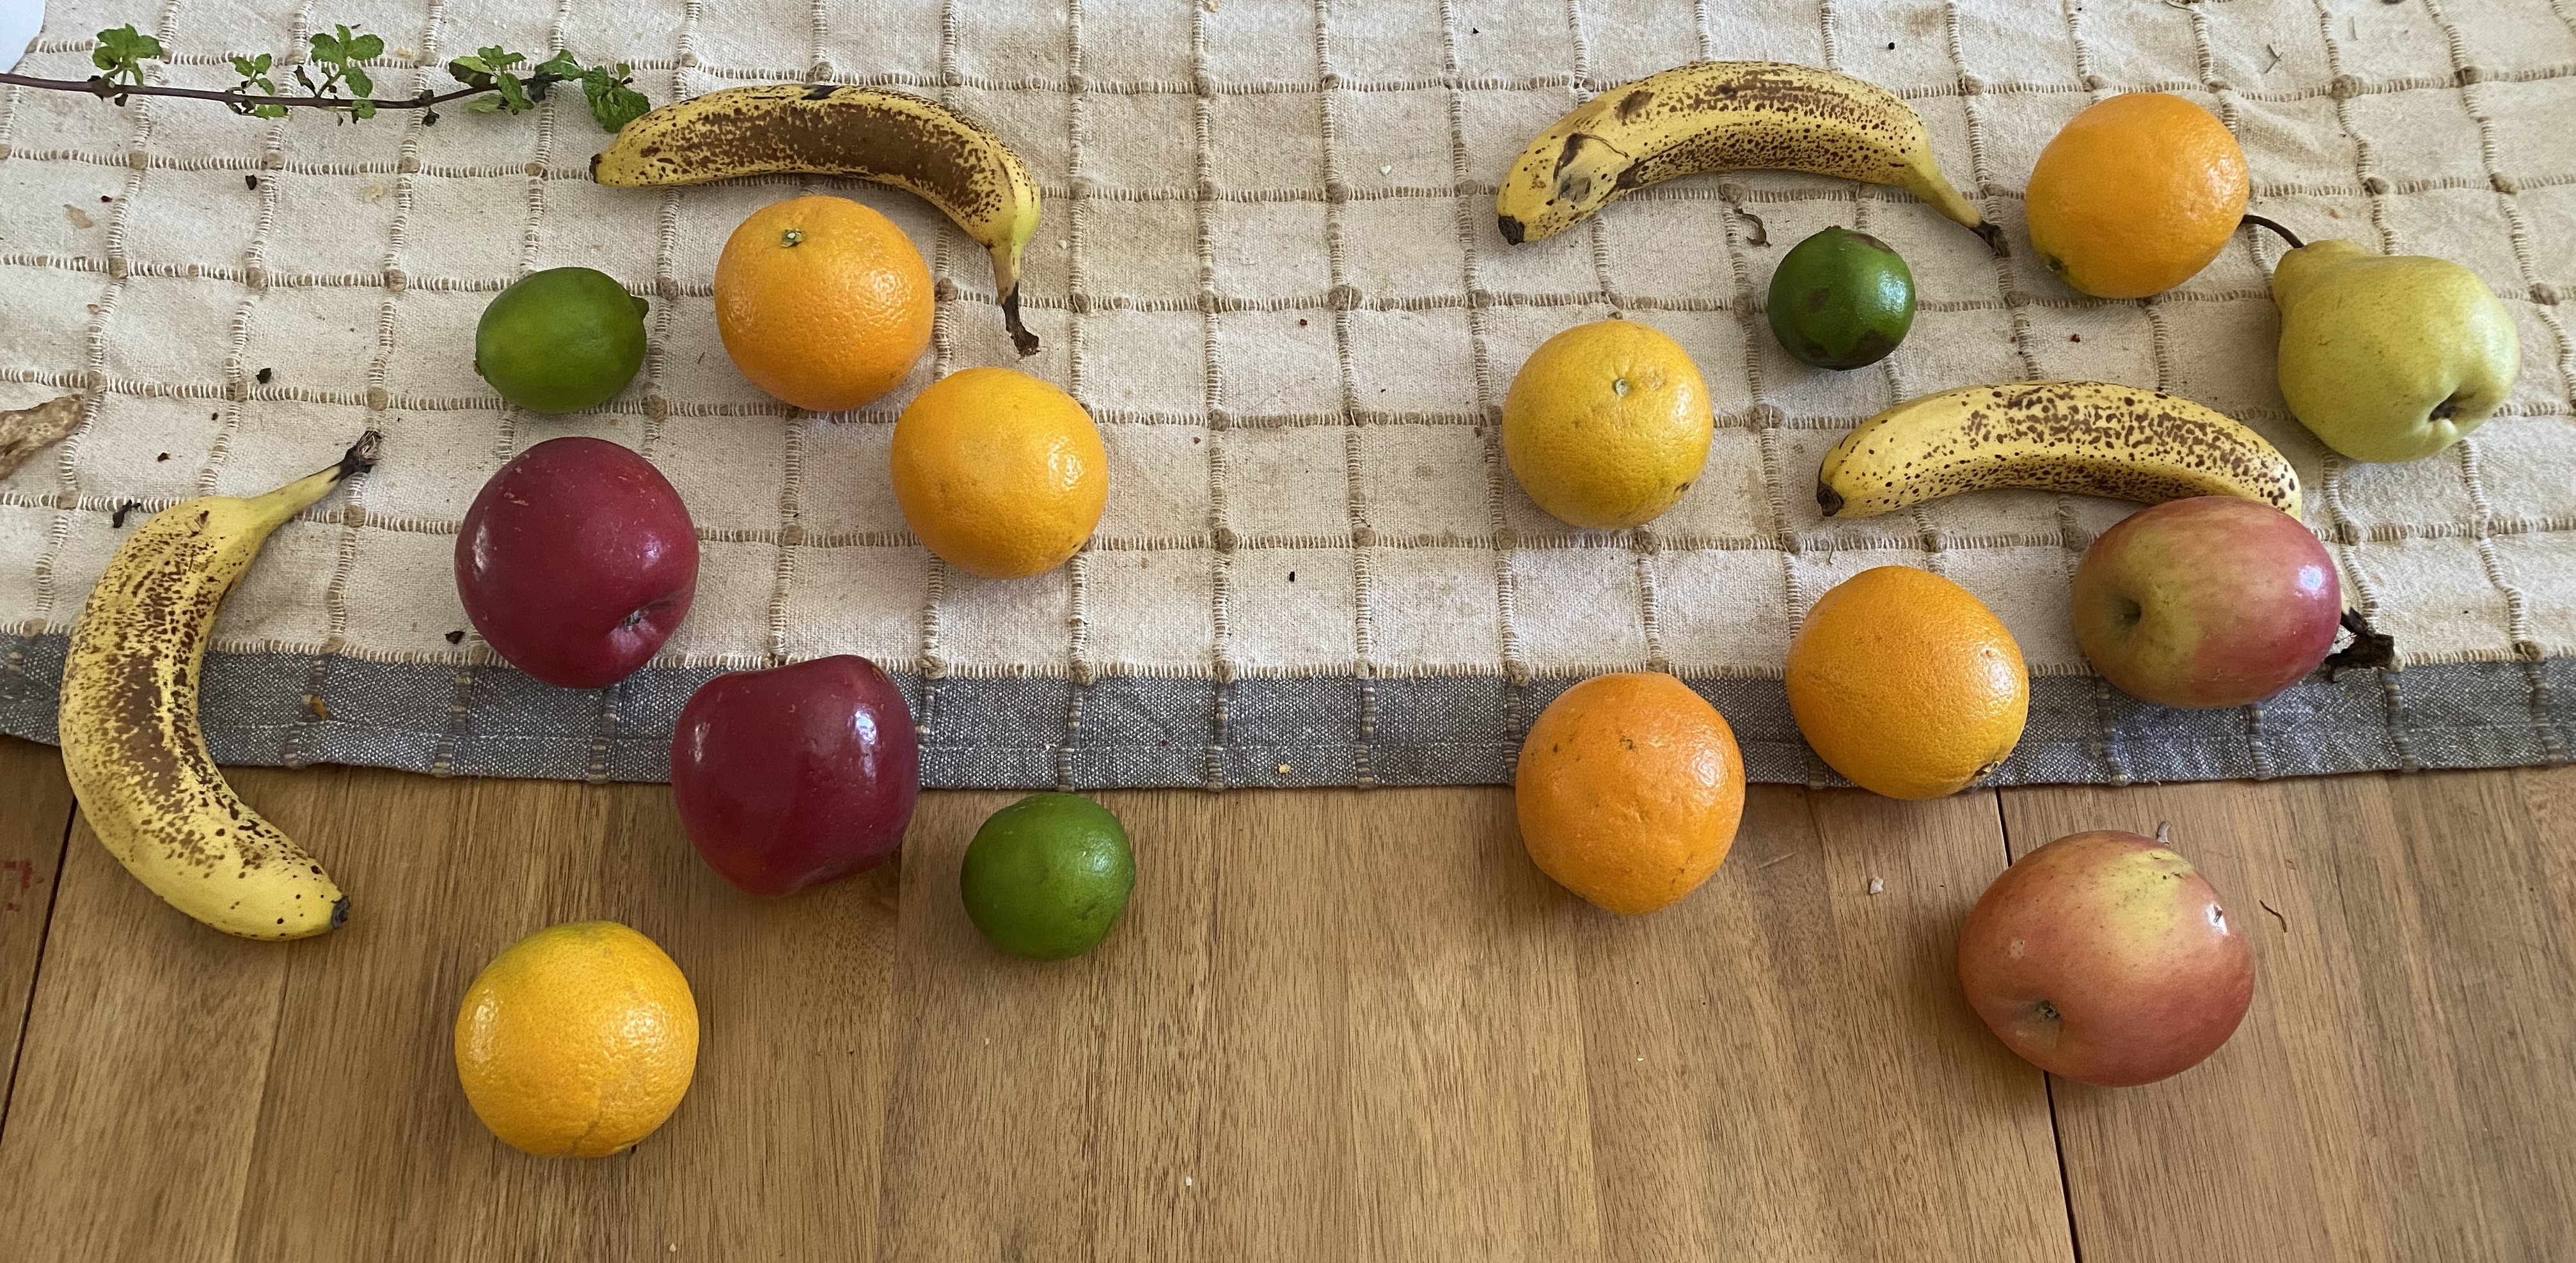
\includegraphics[width=0.48\textwidth]{images/img_2.jpg}
    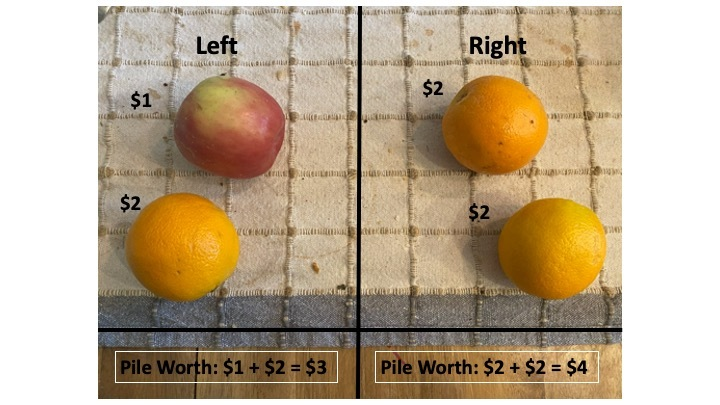
\includegraphics[width=0.48\textwidth]{images/instruction1.jpg}
 \begin{itemize}
	\item Subjects are asked to choose either left pile or right pile under a time pressure.
	\item Each unit fruit is associated with a monetary amount.
	\item Pile value = sum of all fruits.
\end{itemize}
\end{frame}
\subsection{Saliency}

\begin{frame}{Saliency and the Stimuli}
\center
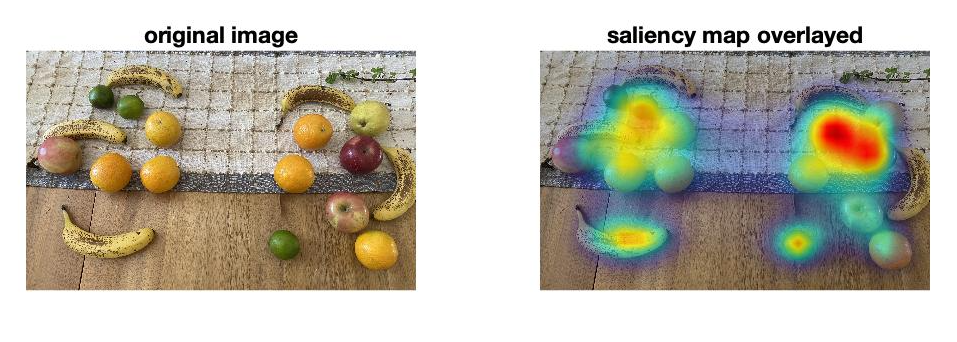
\includegraphics[width=0.48\textwidth,height=3.5cm]{images/heatmap_many2.jpg}
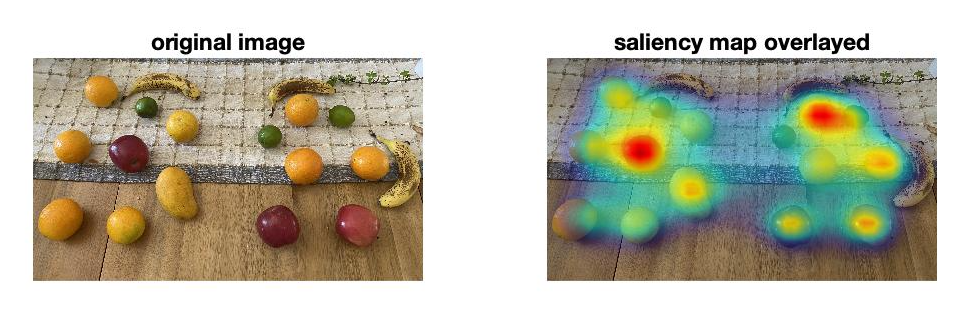
\includegraphics[width=0.48\textwidth,height=3.5cm]{images/twoCenterHeatmap.png}
\begin{itemize}
	\item Saliency measure is determined from SAM algorithm.
	\item SAM is trying to predict the attention allocation of the whole image.
	\item We select only images with one -side saliency center (left example). 
\end{itemize}
\end{frame}


\begin{frame}{Stimulus and Parameters}
	\begin{alertblock}{Two types of stimuli}
		
		\alert{Congruent Condition}: The rewarding pile is also the salient pile.\\
		\alert{Incongruent Condition}: The rewarding pile is the unsalient pile.		
	\end{alertblock}

\begin{itemize}
	\item Each subject: 20 image trials, with 8 congruent trials and 12 incongruent trials. 
	\item Value difference: 10 images below 5 and 10 images ranging from 5-11
	\item Left right balanced for saliency 
	\item Six types of fruits, unit value in integers from 3 to 6.
	\item Time limit: 20 seconds
\end{itemize}
%%NINA: PUT A FLOW CHART HERE
\end{frame}

\section{Result and Analysis}

\begin{frame}{Data}
\begin{itemize}
    \item N=25, on Prolific
    \item Approval rate >75\%
    \item Batch 1) many fruits (reported) Batch 2) four fruits(unreported)
\end{itemize}
\end{frame}


\begin{frame}{Result - Error Rate}
\begin{itemize}
    \item People make more mistakes when saliency property conflicts with reward property. 
    \item Such results holds regardless of valuation difference.
\end{itemize}
\center
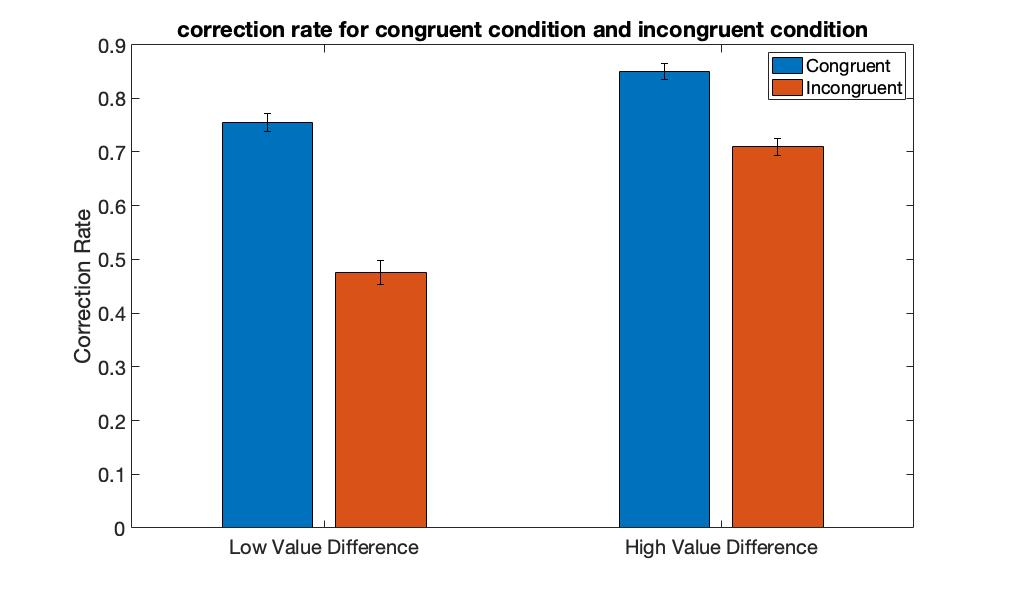
\includegraphics[height = 5cm]{images/errorRateComparison.jpg}
\end{frame}


\begin{frame}
\begin{table}[!htbp] \centering   
\begin{tabular}{@{\extracolsep{5pt}}lD{.}{.}{-3} D{.}{.}{-3} D{.}{.}{-3} D{.}{.}{-3} } 
\\[-1.8ex]\hline 
\hline \\[-1.8ex] 
 & \multicolumn{4}{c}{\textit{Dependent variable: Choice}} \\ 
\hline \\[-1.8ex] 
Rewarding & 0.913^{***} & 0.887^{***} & 0.773^{***} &  \\ 
  & (0.116) & (0.192) & (0.106) &  \\
Salient & 0.876^{***} & 0.857^{***} &  & 0.395^{**} \\ 
  & (0.214) & (0.241) &  & (0.184) \\ 

Value*saliency &  & 0.040 &  &  \\ 
  &  & (0.241) &  &  \\ 

 Constant & -0.492^{***} & -0.474^{**} & -0.013 & 0.090 \\ 
  & (0.159) & (0.192) & (0.106) & (0.128) \\
\hline \\[-1.8ex] 
Observations & \multicolumn{1}{c}{489} & \multicolumn{1}{c}{489} & \multicolumn{1}{c}{489} & \multicolumn{1}{c}{489} \\ 
Log Likelihood & \multicolumn{1}{c}{-296.478} & \multicolumn{1}{c}{-296.464} & \multicolumn{1}{c}{-305.405} & \multicolumn{1}{c}{-331.742} \\ 
Akaike Inf. Crit. & \multicolumn{1}{c}{598.956} & \multicolumn{1}{c}{600.929} & \multicolumn{1}{c}{614.811} & \multicolumn{1}{c}{667.484} \\ 
\hline 
\hline \\[-1.8ex] 
\textit{Note:}  & \multicolumn{4}{r}{$^{*}$p$<$0.1; $^{**}$p$<$0.05; $^{***}$p$<$0.01} \\ 
\end{tabular} 
\end{table} 
\end{frame}

\begin{frame}
\begin{table}[!htbp] \centering 
\begin{tabular}{@{\extracolsep{5pt}}lD{.}{.}{-3} D{.}{.}{-3} D{.}{.}{-3} D{.}{.}{-3} } 
\\[-1.8ex]\hline 
\hline \\[-1.8ex] 
 & \multicolumn{4}{c}{\textit{Dependent variable: correctness}} \\  
\\[-1.8ex] & \multicolumn{1}{c}{(1)} & \multicolumn{1}{c}{(2)} & \multicolumn{1}{c}{(3)} & \multicolumn{1}{c}{(4)}\\ 
\hline \\[-1.8ex] 
 congruency & 0.979^{***} & 0.867^{***} &  & 0.985^{***} \\ 
  & (0.343) & (0.213) &  & (0.219) \\ 
 valueDiff & 0.103^{***} &  & 0.082^{***} & 0.103^{***} \\ 
  & (0.036) &  & (0.029) & (0.030) \\ 
 interaction & 0.001 &  &  &  \\ 
  & (0.066) &  &  &  \\ 
 Constant & -0.071 & 0.457^{***} & 0.383^{**} & -0.073 \\ 
  & (0.214) & (0.120) & (0.162) & (0.192) \\ 
\hline \\[-1.8ex] 
Observations & \multicolumn{1}{c}{489} & \multicolumn{1}{c}{489} & \multicolumn{1}{c}{489} & \multicolumn{1}{c}{489} \\ 
Log Likelihood & \multicolumn{1}{c}{-290.304} & \multicolumn{1}{c}{-296.601} & \multicolumn{1}{c}{-301.186} & \multicolumn{1}{c}{-290.304} \\ 
Akaike Inf. Crit. & \multicolumn{1}{c}{588.607} & \multicolumn{1}{c}{597.203} & \multicolumn{1}{c}{606.371} & \multicolumn{1}{c}{586.608} \\ 
\hline 
\hline \\[-1.8ex] 
\textit{Note:}  & \multicolumn{4}{r}{$^{*}$p$<$0.1; $^{**}$p$<$0.05; $^{***}$p$<$0.01} \\ 
\end{tabular} 
\end{table}
\end{frame}

\begin{frame}
\begin{table}[!htbp] \centering  
\begin{tabular}{@{\extracolsep{5pt}}lD{.}{.}{-3} D{.}{.}{-3} D{.}{.}{-3} } 
\\[-1.8ex]\hline 
\hline \\[-1.8ex] 
 & \multicolumn{3}{c}{\textit{Dependent variable: Response Time}} \\ 
\\[-1.8ex] & \multicolumn{1}{c}{(1)} & \multicolumn{1}{c}{(2)} & \multicolumn{1}{c}{(3)}\\ 
\hline \\[-1.8ex] 
valueDiff & -0.162^{**} & -0.083 & -0.156^{**} \\ 
  & (0.063) & (0.081) & (0.063) \\ 
 congruency & -0.342 & 0.593 &  \\ 
  & (0.460) & (0.763) &  \\ 
interaction &  & -0.198 &  \\ 
  &  & (0.129) &  \\ 
 Constant & 9.048^{***} & 8.632^{***} & 8.882^{***} \\ 
  & (0.441) & (0.517) & (0.380) \\ 
\hline \\[-1.8ex] 
Observations & \multicolumn{1}{c}{489} & \multicolumn{1}{c}{489} & \multicolumn{1}{c}{489} \\ 
R$^{2}$ & \multicolumn{1}{c}{0.014} & \multicolumn{1}{c}{0.018} & \multicolumn{1}{c}{0.012} \\ 
Adjusted R$^{2}$ & \multicolumn{1}{c}{0.010} & \multicolumn{1}{c}{0.012} & \multicolumn{1}{c}{0.010} \\ 
F Statistic & \multicolumn{1}{c}{3.351$^{**}$ (df = 2; 486)} & \multicolumn{1}{c}{3.026$^{**}$ (df = 3; 485)} & \multicolumn{1}{c}{6.153$^{**}$ (df = 1; 487)} \\ 
\hline 
\hline \\[-1.8ex] 
\textit{Note:}  & \multicolumn{3}{r}{$^{*}$p$<$0.1; $^{**}$p$<$0.05; $^{***}$p$<$0.01} \\ 
\end{tabular} 
\end{table}  
\end{frame}


\end{document}